
\newpage
\begin{flushright}
\phantom{}
\vspace{2cm}
\textit{\'A mes amis musiciens, et à ceux qui aiment la musique...}\par
\vspace{1.5cm}
\end{flushright}
\begin{figure}[h]
\begin{center}
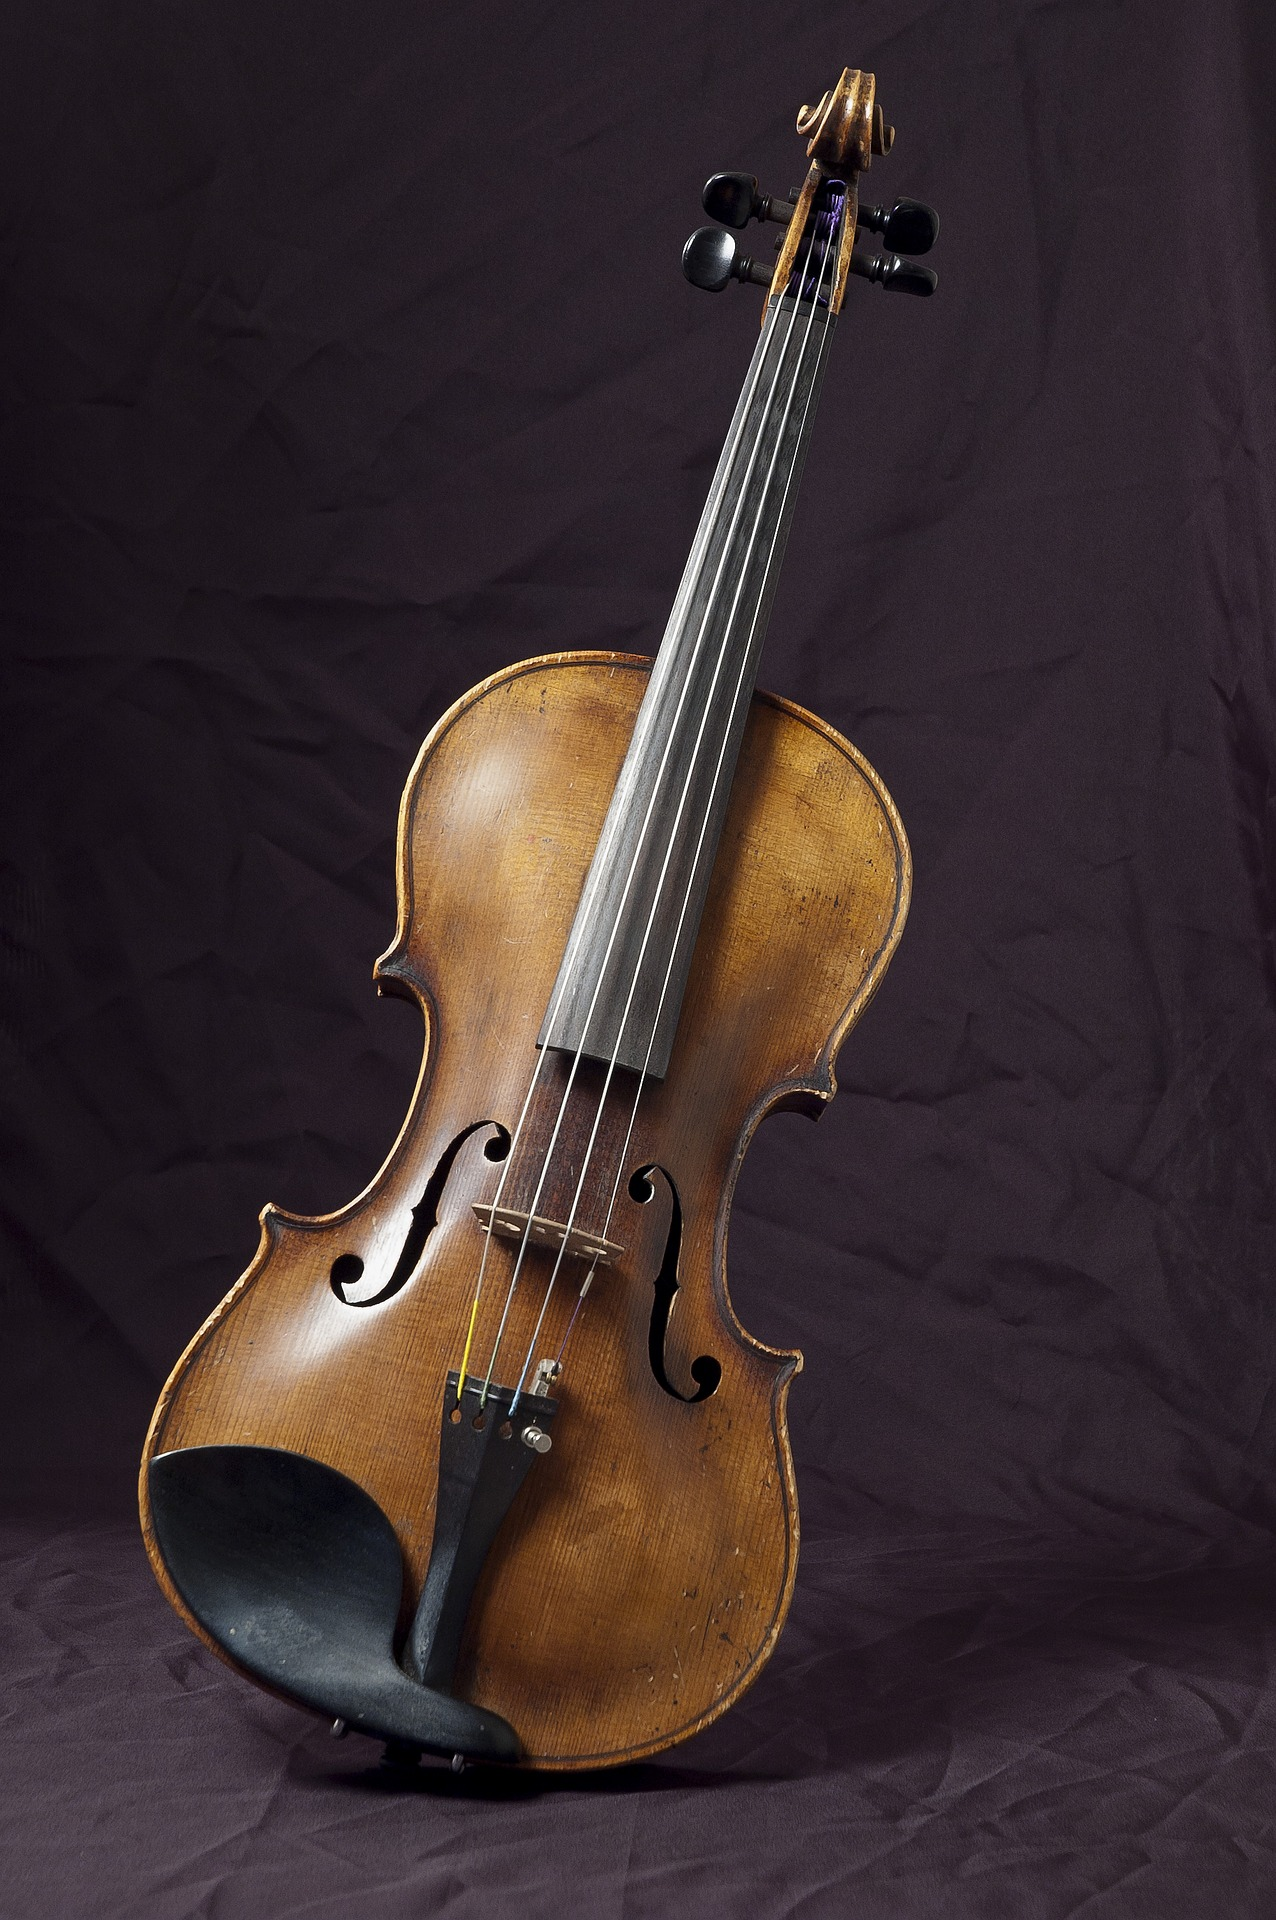
\includegraphics[width=10cm]{images/violin_cover.jpg}
\caption{Un violon muni d'une mentonnière .}
\end{center}
\end{figure}
\par La mentonnière, utilisée pour la première fois au début du XIX\textsuperscript{ème} siècle, est une des premières adaptation du violon au corps du musicien, elle sépare la sueur du violoniste du violon afin de ne pas altérer le vernis à sa surface.

\^A l'image de la mentonnière, mon travail est de perfectionner le ``couple'' du musicien et de son violon.
